\documentclass[dvipsnames,mathserif]{beamer}

%%%%%%%%%%%%%%%%%%%%
%% Personalization of Beamer template
%%%%%%%%%%%%%%%%%%%%
\setbeamertemplate{itemize item}[triangle]
\setbeamercolor{itemize item}{fg=Red}
\setbeamercolor{itemize subitem}{fg=Red}
\setbeamercolor{enumerate item}{fg=Red}
\setbeamercolor{enumerate subitem}{fg=Red}
\setbeamertemplate{enumerate item}[default]
\setbeamertemplate{enumerate subitem}[default]
\setbeamertemplate{frametitle} 
{ 
\begin{centering} \bigskip
\color{Red} \insertframetitle 
\par 
\end{centering} 
} 
\setbeamertemplate{section in toc}{{\color{Red}\inserttocsectionnumber.} {\color{black} \bf \inserttocsection}\\}
\setbeamertemplate{subsection in toc}{$\;\;\;\;\;${\footnotesize {\color{Red}\footnotesize\RIGHTarrow} \inserttocsubsection\\[1mm]}}
\setbeamertemplate{footline}[frame number]
\setbeamertemplate{navigation symbols}{}%remove navigation symbols
\setbeamertemplate{caption}{\insertcaption} 

%%%%%%%%%%%%%%%%%%%%
%% Packages and options
%%%%%%%%%%%%%%%%%%%%

\usepackage{caption,cancel}
\usepackage{multimedia, graphicx} % handling graphics, movies
%\usepackage{amsmath,amsfonts,wasysym,bm} % math, symbols
\usepackage{amsmath,amsfonts,wasysym,bm} % math, symbols
\usepackage{comment} % defines long comment environment
\usepackage{tabularx,booktabs,multirow,array} % packages for nice tables
\usepackage{etex,animate,catchfile} % useful for animations
\captionsetup[figure]{labelformat=empty}% redefines the caption setup
                                % of the figures environment in the
                                % beamer class.


%TiKz
\usepackage{tikz}
\usetikzlibrary{backgrounds,decorations.markings}
\usetikzlibrary{calc}

% Define serif families in math
\usepackage[T1]{fontenc}
\renewcommand*\familydefault{\sfdefault}
%\usepackage{sfmath}

%%%%%%%%%%%%%%%%%%%
%% Define darker colors
%%%%%%%%%%%%%%%%%%%

\definecolor{Blue}{rgb}{0,0,0.9}
\definecolor{Green}{rgb}{0,0.5,0}
\definecolor{Red}{rgb}{0.9,0,0}

\pdfpageattr {/Group << /S /Transparency /I true /CS /DeviceRGB>>}   % fixes transparency issues

%%%%%%%%%%%%%%%%%%%%%
%% Define color of block title %%
%%%%%%%%%%%%%%%%%%%%%

\setbeamercolor{block title}{use=structure,fg=Red}

%%%%%%%%%%%%%%%%%%%%%%
%% Notations %%%%%%%%%%%%
%%%%%%%%%%%%%%%%%%%%%%

\def\Argmax#1{\underset{\substack{#1}}{\mbox{argmax }}}
\def\Argmin#1{\underset{\substack{#1}}{\mbox{argmin }}}


%%%%%%%%%%%%%%%%
%% Defines footnote extra 
%%%%%%%%%%%%%%%%

\makeatletter
% add a macro that saves its argument
\newcommand{\footlineextra}[1]{\gdef\insertfootlineextra{#1}}
\newbox\footlineextrabox

% add a beamer template that sets the saved argument in a box.
% The * means that the beamer font and color "footline extra" are automatically added. 
\defbeamertemplate*{footline extra}{default}{
    \begin{beamercolorbox}[ht=2.25ex,dp=1ex,leftskip=\Gm@lmargin]{footline extra}
    \insertfootlineextra
    \par\vspace{15pt}
    \end{beamercolorbox}
}

\addtobeamertemplate{footline}{%
    % set the box with the extra footline material but make it add no vertical space
    \setbox\footlineextrabox=\vbox{\usebeamertemplate*{footline extra}}
    \vskip -\ht\footlineextrabox
    \vskip -\dp\footlineextrabox
    \box\footlineextrabox%
}
{}

% patch \begin{frame} to reset the footline extra material
\let\beamer@original@frame=\frame
\def\frame{\gdef\insertfootlineextra{}\beamer@original@frame}
\footlineextra{}
\makeatother

%shortcuts
\newcommand{\bi}{\begin{itemize}\setlength{\itemsep}{2mm}}
\newcommand{\ei}{\end{itemize}}

%%%%%%%%%%%%%%%%%%
%% Header from Peter  %%
%%%%%%%%%%%%%%%%%%

\def\subplus{_{\oplus}}
\def\subminus{_{\ominus}}
\def\ie{i.e.\ }
\def\midsection#1{{\subsubsection*{\centering #1}}}
\def\mean{\mathbb{E}}
\def\train{\tilde{x}}
\def\trainlabel{\tilde{y}}
\def\test{x}
\def\testlabel{y}
\def\sp#1{\left< #1\right>}
\def\ind#1{\mbox{\tiny #1}}
\def\indH{\ind{H}}
\def\sgn{\mbox{sgn}}
\def\emprisk{\hat{R}_n}
\def\hypspace{\mathcal{H}}
\def\cost{C}
\def\costperceptron{\cost_{\mbox{\tiny P}}}

\def\conv{\text{conv}}
\def\vH{\mathbf{v}_{\indH}}
\def\train{\tilde{\mathbf{x}}}
\def\Rd{\mathbb{R}^d}
\def\kRBF{k_{\mbox{\tiny RBF}}}
\def\kSP{k_{\mbox{\tiny SP}}}\def\fspace{\mathcal{F}}
\def\spfspace#1{{\sp{#1}}_{\fspace}}

\def\Argmax#1{\underset{\substack{#1}}{\mbox{argmax }}}
\def\Argmin#1{\underset{\substack{#1}}{\mbox{argmin }}}


\def\x{\mathbf{x}}
\def\bbeta{\pmb{\beta}}
\def\hatbeta{\hat{\bbeta}}
\def\image{\mbox{image}}
%\def\span{\mbox{span}}
\def\Xcol{\X^{\mbox{\tiny col}}}
\def\X{\mathbf{X}}
\def\tX{\tilde{\X}}
\def\tXcol{\tX^{\mbox{\tiny col}}}
\def\y{\mathbf{y}}
\def\ty{\tilde{\y}}

\def\seloss{L^{\mbox{\tiny se}}}

\def\r{\mathbf{r}}
\def\btau{\pmb{\tau}}
\def\btheta{\pmb{\theta}}
\def\c{\mathbf{c}}
\def\upj{^{\mbox{\tiny (\,j)}}}
\def\upjplus{^{\mbox{\tiny (\,j+1)}}}
\def\M{\mathbf{M}}
\def\vectheta{\btheta}
\def\assm{a}
\def\bassm{\mathbf{\assm}}
\def\mixture{\pi}


\def\pMeas{\mathbf{M}}
\def\xspace{\mathbf{X}}
\def\skipline{\\ \mbox{ } \\}
\def\tspace{\mathcal{T}}
\def\empdist{\mathbb{F}}
\def\argmax{\mbox{arg}\max}
\def\argmin{\mbox{arg}\min}
\def\simiid{\sim_{\mbox{\tiny iid}}}
\def\posterior{\Pi}
\def\thetaMAP{\hat{\theta}_{\mbox{\tiny MAP}}}
\def\hpspace{\mathcal{H}}
\def\simp{\Delta}
\def\lsep{\\ \mbox{ } \\}

\def\Plimit{P_{\infty}}

\def\noexam{\footlineextra{\sc \textcolor{black}{not examinable.}}}



%%%%%%%%%%%%%%%%%%%%%%%%%%%%%%%%%%%%%%%%%%%%%%%%%%%%%%%%%%%%%%%%
%@@@@@@@@@@@@@@@@@@@@@@@@@@@@@@@@@@@@@@@@@@@@@@@@@@@@@@@@@%
%%%%%%%%%%%%%%%%%%%%%%%%%%%%%%%%%%%%%%%%%%%%%%%%%%%%%%%%%%%%%%%%



%%%%%%%%%%%%%%%%%%%
%% Document begins
%%%%%%%%%%%%%%%%%%%


\begin{document}


\begin{frame}
 
\centering
{\Large \bf \centering \color{Red} Lecture 20: Text Model \\[4mm] }

%{\bf \color{Red} Reading: Sections 8.5,  14.3\\[8mm]}

{\bf GU4241/GR5241 Statistical Machine Learning\\[8mm]}

{\bf Linxi Liu\\ April 20, 2018}

\end{frame}

%%%%%%%%

{\small
\def\t{\mathbf{t}}
\begin{frame}{Categorical Data}
  \begin{block}{Categorical random variable}
    We call a random variable $\xi$ \textbf{categorical} if it takes values
    in a finite set, i.e.\ if $\xi\in \left( 1,\ldots,d \right)$ for
    some $d\in\mathbb{N}$. We interpret the $d$ different outcomes as
    $d$ separate \emph{categories} or classes.
  \end{block}

\begin{block}{Category probabilities}
    Suppose we know the probability $t_j=\mbox{Pr}\left( \xi =
    j \right)$ for each category $j$. Then
    \begin{equation*}
      t_j \geq 0 \qquad \text{ and } \qquad
      \sum_{j=1}^d t_j = 1
    \end{equation*}

 We can represent the distribution of $\xi$ by the vector
    $\t=(t_1,\ldots,t_j) \in \mathbb{R}^d$. In other words, we can
    parameterize distributions of categorical variables by vectors $\mathbf{t}$.
\end{block}
  
\end{frame}

\def\H{\mathbf{H}}
\begin{frame}{Samples of Size $n$}
  \begin{block}{A single sample}
    We can represent a single sample as a vector, e.g.
    \begin{equation*}
      (0,1,0,0,0) \qquad \text{ if } \quad  d=5 \quad \text{ and }
      \quad \xi=2\;.
    \end{equation*}
    (Recall the assignments in EM.)
  \end{block}
  \begin{block}{$n$ samples}
    A sample of size $n$ is a vector of counts, e.g.
    \begin{equation*}
      (2,5,1,3,0) 
    \end{equation*}
    We denote the counts by $H_j$ and write
    \begin{equation*}
      \H:=(H_1,\ldots,H_d) \qquad \text{ with } \qquad \sum_{j=1}^d H_j = n\;.
    \end{equation*}
  \end{block}
\end{frame}

%%%%%%%%%%%%%%%%%%%%%%%%%%%%%%%%%%%%%%%%%%%

\def\t{\mathbf{t}}
\begin{frame}{Multinomial Distribution}
  \begin{block}{Modeling assumption}
    The $n$ observations of $\xi$ are independent, and the probability
    for $\xi=j$ in each draw is $t_j$. What is the probability of
    observing the sample $H=(H_1,\ldots,H_j)$?
  \end{block}
  \begin{block}{Multinomial distribution}
    Answer: The probability is
    \begin{equation*}
      P(\H|\t)=\frac{n!}{H_1!\cdots H_d!}\prod_{j=1}^d t_j^{H_j}
      =
      \frac{n!}{H_1!\cdots H_d!}\exp\Bigl(\sum_{j=1}^d H_j\log(t_j)\Bigr)
    \end{equation*}
    Recall: $n! = 1\cdot 2\cdot 3\cdot\ldots\cdot n$
  \end{block}
  \textbf{Note:} The assingment variables $M_i$ in a finite mixture
  model are multinomially distributed with $n=1$ and $\theta=(c_1,\ldots,c_k)$.
  \begin{block}{As an exponential family}
    The form of $P$ above shows that the multinomial is an EFM with
    \begin{equation*}
      S(\H):=\H \qquad h(\H):=\frac{n!}{H_1!\cdots H_d!} \qquad \theta_j:=\log t_j 
      \qquad Z(\theta):=1 \;.
    \end{equation*}
  \end{block}
\end{frame}

\begin{frame}{Explanation}
    \begin{itemize}
    \item In one draw, the probability of observing $\xi=j$ is $t_j$.
    \item In $n$ draws, the probability of $n$ times observing $\xi=j$
      is $t_j^n$.
    \end{itemize}
    Suppose we have $n=3$ observation in two categories. How many ways are
    there to observe exactly two observations in category 1? Three:
{\scriptsize
    \begin{center}
    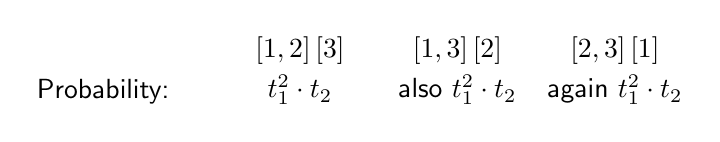
\begin{tikzpicture}
      \node at (-2,0) {$[1,2]\, [3]$};
      \node at (0,0) {$[1,3]\, [2]$};
      \node at (2,0) {$[2,3]\, [1]$};

      \node at (-4.5,-0.52) {Probability:};
      \node at (-2,-0.5) {$t_1^2\cdot t_2$};
      \node at (0,-0.5) {also $t_1^2\cdot t_2$};
      \node at (2,-0.5) {again $t_1^2\cdot t_2$};
    \end{tikzpicture}
    \end{center}
}
    The total probability of $H_1=2$ and $H_2=1$ is $3\cdot t_1^2\cdot t_2$.
    \begin{itemize}

    \item The number of ways that $n$ elements can be subdivided into
      $d$ classes with, $H_j$ elements falling into class $j$, is
      precisely
      \begin{equation*}
        \frac{n!}{H_1!\cdots H_d!}
      \end{equation*}
    \end{itemize}
    In the multinomial formula:
\vspace{-1mm}
    \begin{equation*}
      P(\H|\t)=\underbrace{\frac{n!}{H_1!\cdots H_d!}}_{\text{\#
          combinations}}\underbrace{\prod_{j=1}^d
        t_j^{H_j}}_{\text{probability of \emph{one} combination}}
    \end{equation*}
\end{frame}

\begin{frame}{Parameter Estimation}
  \begin{block}{MLE}
    The maximum likelihood estimator of $\t$ is
    \begin{equation*}
      \hat{\t}=(\hat{t}_1,\ldots,\hat{t}_d)
      :=\frac{1}{n}(H_1,\ldots,H_d) \;.
    \end{equation*}
  \end{block}
\end{frame}

\def\simp{\triangle}
\begin{frame}{Multinomial Parameters and Simplices}
  \begin{columns}
    \begin{column}{0\textwidth}
    \end{column}
    \begin{column}{0.7\textwidth}
\vspace{-3mm}
      \begin{block}{The simplex}
      The set of possible parameters of a multionmial distribution is
\vspace{-2mm}
{\scriptsize
      \begin{equation*}
        \simp_d:=\lbrace \t \in \mathbb{R}^d \,|\,
        t_j\geq 0 \text{ and }\sum t_j =1 \rbrace
      \end{equation*}
}
%\vspace{-2mm}
      $\simp_d$ is a subset of $\mathbb{R}^d$ and is called the
      \textbf{$d$-simplex}, or the \textbf{standard simplex in
        $\mathbb{R}^d$}.
      \end{block}
\vspace{-2mm}
      \begin{block}{Interpretation}
\vspace{-3mm}
        \begin{itemize}
      \item Each point in e.g.\ $\simp_3$ is a distribution on 3
        events.
\vspace{-2mm}
      \item Each extreme point (corner) correspond to one category $j$
        and is the distribution with $t_j=1$.
\vspace{-2mm}
      \item The edges of $\simp_3$ are the distributions under which
        only 2 events can occur. (The category corresponding to the
        opposite corner has zero probability.)
\vspace{-2mm}
      \item The inner points are distributions under which all
        categories can occur.
        \end{itemize}
      \end{block}
    \end{column}
    \begin{column}{0.4\textwidth}
      \begin{center}
        \input{../figures/fig_simplex.tex}
      \end{center}
    \end{column}
  \end{columns}
\end{frame}

%%%%%%%%%%%%%%%%%%%%%%%%%%%%%%%%

\begin{frame}{Example 1: Local Image Histograms}
  \begin{block}{Extracting local image statistics}
    \begin{columns}
      \begin{column}{0\textwidth}
      \end{column}
      \begin{column}{0.5\textwidth}
        \begin{tikzpicture}
          \node {\includegraphics[width=4cm]{../figures/sima.png}};
          \draw[red] (-1,1) rectangle (-1.1,1.1);
          \node (patch) at (3,1) {\includegraphics[width=1cm]{../figures/sima_patch.png}};
          \draw[red] ($(patch.south west)+(0.11,0.11)$)--(-1,1);
          \draw[red] ($(patch.north west)+(0.11,-0.11)$)--(-1,1.1);
        \end{tikzpicture}
      \end{column}
      \begin{column}{0.5\textwidth}
        \begin{enumerate}
        \item Place a small window (size $l\times l$) around location in image.
        \item Extract the pixel values inside the image. If the grayscale values are e.g. $\lbrace 0,\ldots,255\rbrace$,
          we obtain a histogram with 256 categories.
        \item Decrease resolution by binning; in Homework 4, we decrease from 256 to 16 categories.
        \end{enumerate}
      \end{column}
    \end{columns}
  \end{block}
\vspace{-2mm}
  \begin{block}{Resulting data}
\vspace{-6mm}
    \begin{equation*}
      \H=(H_1,\ldots,H_{16})
      \qquad\text{ where }\qquad
      H_j=\#\text{ pixel values in bin $j$ }\;.
    \end{equation*}
  \end{block}
\vspace{-2mm}
  Since $256/16=8$, bin $j$ represents the event
  \begin{equation*}
    \text{ pixel value }\in\lbrace (j-1)\cdot 8,\ldots, j\cdot 8 -1\rbrace \;.
  \end{equation*}
\end{frame}

\begin{frame}{Example 1: Local Image Histograms}
  \begin{block}{Multinomial model}
    We can model the data by a multinomial distribution
    $P(\H|\mathbf{t},n=l^2)$. Then
    \begin{equation*}
      t_j=\mbox{Pr}\lbrace \xi=j \rbrace =
      \mbox{Pr}\lbrace \text{ grayscale value falls in bin $j$ }\rbrace \;.
    \end{equation*}
  \end{block}
  \begin{block}{Homework: Multinomial clustering}
    \begin{columns}
      \begin{column}{0\textwidth}
      \end{column}
      \begin{column}{0.3\textwidth}
        \begin{center}
        \includegraphics[width=3cm]{../figures/sima.png}
        \end{center}
      \end{column}
      \begin{column}{0.7\textwidth}
        \begin{itemize}
          \item The probability of e.g. bin 1 (dark pixels) clearly varies between locations in the image.
          \item Consequence: A single multinomial distribution is not a good representation of this image.
          \item In HW 5, the image is represented by a mixture of multinomials which is estimated using EM.
        \end{itemize}
      \end{column}
    \end{columns}
  \end{block}
\end{frame}

%%%%%%%%%%%%%%%%%%%%%%%%%%%%%%%%%%%%%%%%

\begin{frame}{Text Data}
  \begin{block}{Setting}
    Data set: A huge set of text documents (e.g.\ all books in a
    library). The entire set of texts is called a \textbf{corpus}.
    \lsep
    Can we learn models from text which describe natural language?
  \end{block}
  \begin{block}{Terminology}
    We have to distinguish occurences of words in a document and
    \emph{distinct} words in the dictionary. We refer to words
    regarded as entries of the dictionary
    as \textbf{terms}.
  \end{block}
\end{frame}

\begin{frame}{Example 2: Simple Text Model}
  \begin{block}{Data}
    Suppose our data is a text document. We are given a dictionary which contains all terms occurring in the document.
  \end{block}
  \begin{block}{Documents as vectors of counts}
    We represent the document as
    \begin{equation*}
      \H=(H_{1},\ldots,H_{d})
      \qquad
      \text{ where }
      H_{j}=\#\text{ occurences of term $j$ in document.}
    \end{equation*}
    Note: \begin{itemize}
    \item $d$ is the number of all terms (distinct words) in the dictionary
      \ie $d$ is identical for all documents.
    \item $n=\sum_j H_j$ can change from document to document.
    \end{itemize}
  \end{block}
\end{frame}

%%%%%%%%%%%%%%%%%%%%%%%%%%%%%%%%%%%

\begin{frame}{Example 2: Simple Text Model}
  \begin{block}{Multinomial model}
    To define a simple probabilistic model of document generation, we 
    can use a multinomial distribution $P(\H|\mathbf{t},n)$. That means:
    \begin{itemize}
    \item Each word in the document is sampled independently of the other words.
    \item The probabilities of occurrence are
      \begin{equation*}
        \mbox{Pr}\lbrace \text{ word } = \text{ term $j$ }\rbrace = t_j\;.
      \end{equation*}
    \end{itemize}
  \end{block}
  \begin{block}{Implicit assumption}
    The assumption implicit in this model is that the probability of observing a document
    is completely determined by how often each term occurs;  the order of words
    does not matter. This is called the \textbf{bag-of-words
      assumption}.
  \end{block}
\end{frame}

\begin{frame}{Context}
  \begin{block}{Task}
    Can we predict the next word in a text?
  \end{block}
  \begin{block}{Context}
    In language, the co-occurence and order of words is highly
    informative. This information is called the \textbf{context} of a
    word.\\
    \textbf{Example:} The English language has over 200,000 words. 
    \begin{itemize}
    \item If we choose any word at random, there are over 200,000
      possibilities.
    \item If we want to choose the next word in
      \begin{center}
        There is an airplane in the $\_\_$
      \end{center}
      the number of possibilities is \emph{much} smaller.
    \end{itemize}
  \end{block}
\vspace{-2mm}
  \begin{block}{Significance for statistical methods}
    Context information is well-suited for machine learning: By
    parsing lots of text, we can record which words occur together and
    which do not.\\
    \vspace{3mm}
    The standard models based on this idea are called \emph{$n$-gram models}.
  \end{block}
\end{frame}

\def\Prob{\mbox{Pr}}
\begin{frame}{Bigram Models}
  \begin{block}{Bigram model}
    A bigram model represents the conditional distribution
    \begin{equation*}
      \Prob(\text{word}|\text{previous word}) = :\Prob(w_l|w_{l-1}) \;,
    \end{equation*}
    where $w_l$ is the $l$th word in a text.
  \end{block}
  \begin{block}{Representation by multinomial distributions}
    A bigram model is a \emph{family} of $d$ multinomial distributions,
    one for each possible previous word.
  \end{block}
  \begin{block}{Estimation}
    For each term $k$, find all terms in the corpus which are
    preceeded by $k$ and record their number of occurences in a vector
    \begin{equation*}
      \H_k=(H_{k1},\ldots,H_{kd}) \ \text{ where } H_{kj}=\text{number of times term $j$ follows on term $k$}
    \end{equation*}
    Then compute the maximum likelihood estimate $\hat{\t}_k$ from
    the sample $\H_k$.  
    
    \textbf{Note:} Both $j$ and $k$ run through $\lbrace
    1,\ldots,d\rbrace$.
  \end{block}
\end{frame}

%%%%%%%%%%%%%%%%%%%%%%%%%%%%%%

\begin{frame}{$N$-Gram Models}
  \begin{block}{Multinomial representation of bigram}
    The distributions in the bigram model are:
\vspace{-1mm}
    \begin{equation*}
      \Prob(\text{word}=j|\text{previous word}=k)
      =
      P(H_j=1|\hat{\t}_k, n=1)
    \end{equation*}
    where $P$ is the multinomial distribution. The entire bigram model
    is the set
    \begin{equation*}
      \lbrace P(\,.\,|\hat{\t}_k, n=1) \,|\, k=1,\ldots,d \rbrace
    \end{equation*}
  \end{block}
\vspace{-3mm}
  \begin{block}{$N$-gram models}
    More generally, a model conditional on the $(N-1)$ previous words
    \begin{equation*}
      \Prob(w_l|w_{l-1},\ldots,w_{l-(N-1)})
    \end{equation*}
    is called an \textbf{$N$-gram model} (with the predicted word,
    there are $N$ words in total).
  \end{block}
  \begin{block}{Unigrams}
    The special case $N=1$ (no context information) is the
    simple multinomial word probability model which we
    discussed first. This model is also called a \textbf{unigram
      model}.
  \end{block}
\end{frame}

%%%%%%%%%%%%%%%%%%%%%%%%%%%

\begin{frame}{Learning Shakespeare 1}
%{\scriptsize
\vspace{2mm}
  \begin{columns}[t] 
    \begin{column}{0.5\textwidth}
      \vspace{-0.8cm}
      \begin{center}
        \textbf{Unigram Model}
      \end{center}
      To him swallowed confess hear both. Which. Of save on trail for are ay
      device and rote life have 
      \lsep
      Every enter now severally so, let 
      \lsep
      Hill he late speaks; or! a more to leg less first you enter
      \lsep   
      Are where exeunt and sighs have rise excellency took of.. Sleep
      knave we. near; vile like
    \end{column}
    \begin{column}{0.5\textwidth}
      \vspace{-0.8cm}
      \begin{center}
        \textbf{Bigram Model}
      \end{center}
      What means, sir. I confess she? then all sorts, he is trim,
      captain. 
      \lsep
      Why dost stand forth thy canopy, forsooth; he is this
      palpable hit the King Henry. Live king. Follow. 
      \lsep
      What we, hath got so
      she that I rest and sent to scold and nature bankrupt, nor the first
      gentleman? 
      \lsep
      Enter Menenius, if it so many good direction found'st thou
      art a strong upon command of fear not a liberal largess given away,
      Falstaff! Exeunt
    \end{column}
  \end{columns}
%}
  \vspace{2cm}
  \footlineextra{From Jurafsky and Martin, "Speech and Language
    Processing", 2009.}
\end{frame}

%%%%%%%%%%%%%%%%%%%%%%%%%%%%%%%%

\begin{frame}{Learning Shakespeare 2}
%\vspace{2mm}
  \begin{columns}[t]
    \begin{column}{0.5\textwidth}
      \vspace{-1cm}
      \begin{center}
        \textbf{Trigram Model}
      \end{center}
      Sweet prince, Falstaff shall die. Harry of Monmouth's grave. 
      \lsep
      This shall forbid it should be branded, if renown made it empty. 
      \lsep
      Indeed the duke; and had a very good friend. 
      \lsep
      Fly, and will rid me these news of price. Therefore the sadness of
      parting, as they say, 'tis done.
    \end{column}
    \begin{column}{0.5\textwidth}
      \vspace{-1cm}
      \begin{center}
        \textbf{Quadrigram Model}
      \end{center}
      King Henry. What! I will go seek the traitor Gloucester. Exeunt some
      of the watch. A great banquet serv'd in; 
      \lsep
      Will you not tell me who I am? 
      \lsep
      It cannot be but so.
      \lsep
      Indeed the short and the long. Marry, 'tis a noble Lepidus.
    \end{column}
  \end{columns}
 \footlineextra{From Jurafsky and Martin, "Speech and Language
   Processing", 2009.}
\end{frame}

\begin{frame}{Complexity of $N$-Gram Models}
  \begin{block}{Enumerating contexts}
    An $N$-gram model considers ordered combinations of $N$ terms
    (=\emph{distinct} words).
    Say a corpus contains 100,000 words. Then there are
    \begin{equation*}
      100000^N = 10^{5N}
    \end{equation*}
    possible combinations. 
  \end{block}
  \begin{block}{Naive estimate}
    If we require on average $n$ observations per combination to get a
    reliable estimate, we would need a corpus containing $n\cdot
    10^{5N}$ words.
  \end{block}
  \begin{block}{Consequence}
    In practice, you typically encountner bigrams or
    trigrams. Research labs at some internet companies have
    reported results for higher orders.
  \end{block}
\end{frame}

\begin{frame}{Clustering Text}
  \begin{block}{Task}
    Suppose we have a corpus consisting of two types of text, (1)
    cheap romantic novels and 
    (2) books on theoretical physics. Can a clustering algorithm with
    two clusters
    automatically sort the books according to the two types?\\
    \vspace{2mm}
    (We will see that there is more to this than solving artificial
    sorting problems.)
  \end{block}
  \begin{block}{Clustering model}
    We assume the corpus is generated by a  multinomial mixture model
    of the form 
\vspace{-1mm}
    \begin{equation*}
      \pi(\H)=\sum_{k=1}^K c_k P(\H|\t_k)\;,
    \end{equation*}
    \ie each component $P(\H|\t_k)$ is multionmial.\\
    \textbf{However:} We are now considering \textbf{documents} rather
    than individual words.
  \end{block}
  \begin{block}{Estimation}
    Apply EM algorithm for multinomial mixture models.
  \end{block}
\end{frame}


\begin{frame}{Intepretation: Topics}
  \begin{block}{Thought experiment}
    Say we run a mixture of two multinomial distributions on the cheap
    romantic novels and theoretical physics textbooks.\\
    \vspace{3mm}
    Outcome:
    \begin{itemize}
    \item Each cluster will roughly represent one of the two topics.
    \item The two parameter vectors $\t_1$ and $\t_2$
      represent distributions of words in \emph{texts of the
        respective topic}.
    \end{itemize}
  \end{block}
  \begin{block}{Word distributions as topics}
    This motivates the interpretation of clusters as topics.
    \begin{equation*}
      \t_k = \text{ distribution of words that characterizes topic
        $k$ }
    \end{equation*}
    Language models derived from this idea are called \textbf{topic models}.
  \end{block}
\end{frame}





}

\end{document}


   
  











